% Chapter 3

\chapter{Development} % Write in your own chapter title
\label{chap:development}
\lhead{Chapter 3. \emph{Development}} % Write in your own chapter title to set the page header
\begin{flushright}
\textit{``For me, open source is a moral thing.''} \\ Matt Mullenweg
\end{flushright}

In this chapter, we introduce our contribution to the dynamic program analysis. As explained in the introduction the aim is to develop a proof-to-concept system and all the steps to achieve it will be presented in details including the Setup, Data capture model, Data model and its user interface.


\section{Proposed solution}
While working on a growing project, there is always a point where it becomes difficult to keep an eye on all the variables. In order to give the programmer an overview of the variables evolution, this work is aiming to propose a proof-to-concept system which will not only monitor the data evolution, but also give the possibility to compare the gathered data between different runs.

To achieve such a system, the project is going to be separated in three different parts which will constitute the system. First, a data capture model will monitor all the needed variables and their evolution during the execution of the reviewed program. Then a data model will be created and backup procedure will be implemented to store the data in this model. Finally, a web-application will process the extracted data and show them for reviewing the results. Each mentioned part is exposed in the development section.

\section{Environment}
This section describes environment installed and used for the development and deployment phase. 

\subsection{Development system}
The development machine was installed on the GNU/Linux distribution Fedora 24 with Python 3.4 and MongoDB 3.2. The chosen IDE was PyCharm academic edition version 2015 and then 2016. PyCharm is a very complete IDE which supports among others Python web frameworks, database support, code inspection. In order to optimize the development management, the GitHub online tool was chosen as version control repository. The details about the technologies are presented under the next point.

\subsection{Technologies}
For the project 4 main technologies were chosen in order to develop the required features. 

First the data is captured in \textit{Python} with the help of the integrated Debugger Framework. Python is a widely used high level programming language which has seen these last year an increasing enthusiasm around it, especially for web based applications. Thanks to the dynamic nature of Python, which includes a dynamic type system, the real-time collection of object is a pretty straightforward process and therefore it made plenty sense to use it in our project. More over Python offers good compatibility with other programming language since there are a lot of bindings available. For this project, the newest version 3 of the programming language was chosen because of the better handling of encoding.

Secondly, the extracted data is stored in a \textit{MongoDB} Database. MongoDB is a document-oriented database which enters in the new categorie of No-SQL database systems. MongoDB has the advantage to use JSON-like documents with schemas which was a clever choice to store the heterogeneous extracted data.

Finally, the used interface was built with the help of \textit{Python}, \textit{Html/CSS} and \textit{Javascript}. As already said, Python is now an interesting language to develop web applications and was used here, with the help of the Flask framework, for the server side process. HTML/CSS and Javascript were used for the presentation of the results.

Each module of the solution is presented in details in the section 3.3. 

\subsection{Deployment}
The deployment during the development of the solution was tested on virtual machine server under Ubuntu Server 14.04. The server is provided by the Department of Informatics at the University of Fribourg and is accessible internally at \url{http://diufpc115.unifr.ch/}. This server will also be used for the experiments in the chapter 5. 

In order to deploy regularly the newest version of the ongoing work an automation server named Jenkins was configured. Jenkins was charged to fetch every day the latest prototype on the GitHub repository, create a package of it and install it on the server. If during this process a bug occurred, an e-mail to the interested persons was sent.

\bigskip

\begin{figure}[h!]
  \centering
    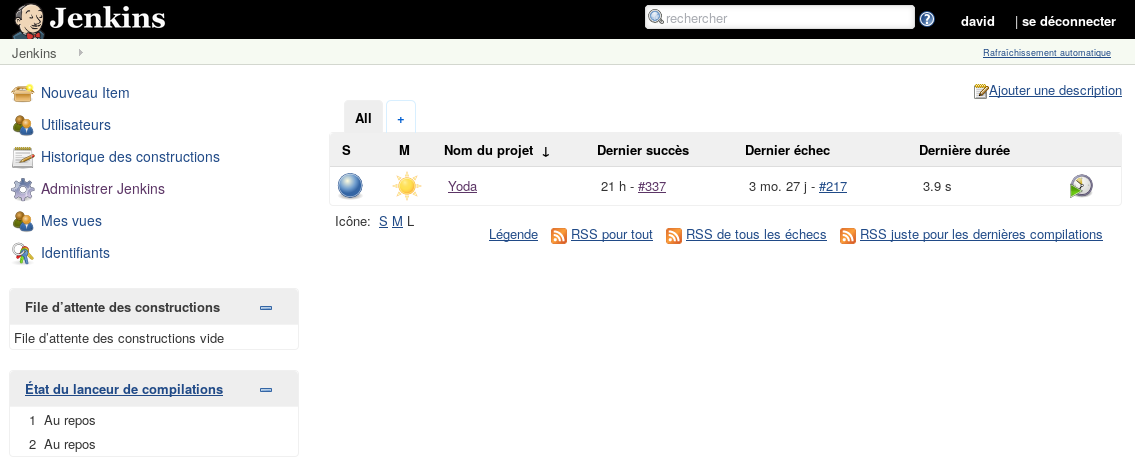
\includegraphics[width=\textwidth]{figures/jenkins.png}
    \caption{The Jenkins home page}
    \label{fig:jenkins}
\end{figure}

\section{Development}

In the following point, the details of the development phase is explained in details.



\subsection{Data capture model}
Base code from roman
Basics of the pydebugger
Some code citations

\subsection{Data model}
how you store data in a database

\subsection{User interface}

\section{Concluding remarks}
